
\section{Method: When to Apply Learned Correction}
\label{sec:method}

\begin{figure}[t]
  \centering
  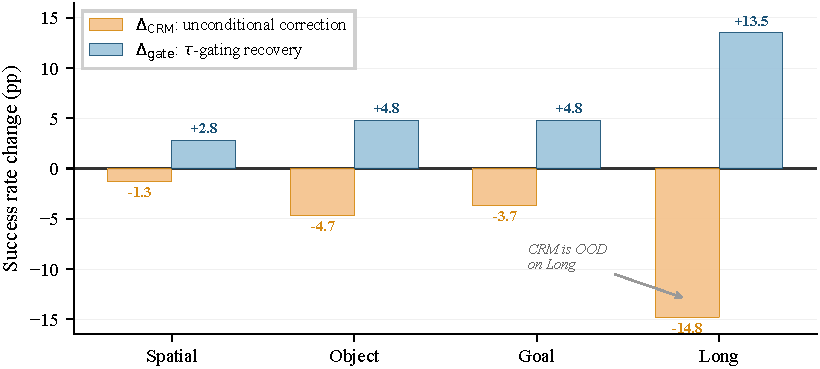
\includegraphics[width=\linewidth]{fig_teaser.pdf}
  \caption{Degradation from unconditional correction ($\Delta_{\mathrm{CRM}}$, orange) vs.\ recovery from calibrated $\tau$-gating ($\Delta_{\mathrm{gate}}$, blue) across four LIBERO suites on SmolVLA. Unconditional CRM correction degrades all suites (up to $-$14.8\,pp on Long, where the CRM is out-of-distribution); $\tau$-gating recovers nearly all degradation by restricting correction to high-uncertainty steps.}
  \label{fig:teaser}
\end{figure}

We propose a calibrated gating pipeline for frozen flow-matching VLAs (Figure~\ref{fig:pipeline}). The calibration is based on held-out percentile thresholds of pairwise distances; it does not implement formal conformal prediction guarantees~\cite{angelopoulos2023gentle}. Since unconditional learned correction degrades all evaluated suites (Section~\ref{sec:failure_modes}), the pipeline uses a $K{=}2$ pairwise distance to decide per step whether correction is safe. At each control step, the pairwise $L_2$ distance between two stochastic action samples forms an uncertainty score; confident steps output the selected sample directly, while uncertain steps apply a learned residual correction via a lightweight Correction Residual Module (CRM). The base VLA is never retrained.

\subsection{Problem Setup}
\label{sec:problem_setup}

Let $\pi_\theta$ be a frozen flow-matching VLA that, given an observation $o_t$ (image, language instruction, proprioceptive state), generates action chunks of length $C{=}50$ in $\mathbb{R}^{d \times C}$ with $d{=}6$ (3 translation + 3 rotation). Under receding-horizon execution, only the first $H{=}5$ steps of each chunk influence the robot before re-planning, so we discard the remainder. The gripper dimension is handled separately via direct thresholding and is excluded from the pipeline.

Each forward pass of $\pi_\theta$ produces a stochastic action sample; querying independently $K$ times yields $K$ candidate chunks. Our goal is to produce a single action more accurate than any individual sample, with no changes to $\pi_\theta$. The method applies to any stochastic generative policy---including diffusion policies~\cite{chi2023diffusion_policy} and flow-matching VLAs---that produces diverse action samples (Appendix~\ref{sec:applicability}).

\subsection{Multi-Sample Selection}
\label{sec:selection}

We draw $K$ action chunks from $\pi_\theta$ via independent flow-matching rollouts and truncate each to $H{=}5$ steps, yielding samples $\{a_h^{(k)}\}_{k=1}^K$ with $a_h^{(k)} \in \mathbb{R}^d$ for horizon step $h = 1, \dots, H$. For each step, we compute the sample mean $\boldsymbol{\mu}_h = \frac{1}{K}\sum_{k=1}^K a_h^{(k)}$ and select the sample with the smallest total $L_2$ distance to the mean across all horizon steps:
\begin{equation}
  a_{\mathrm{base}} = \argmin_{k \in \{1,\dots,K\}} \sum_{h=1}^{H} \bigl\|a_h^{(k)} - \boldsymbol{\mu}_h\bigr\|_2^2.
  \label{eq:argmin}
\end{equation}
Unlike the element-wise mean, which can blend incompatible modes, the argmin returns an actual sample and preserves within-sample temporal coherence. At $K{=}2$, the argmin-to-centroid cost is identical for both samples ($\|a^{(1)} - \boldsymbol{\mu}\| = \|a^{(2)} - \boldsymbol{\mu}\| = \|a^{(1)} - a^{(2)}\|/2$), so selection reduces to a deterministic index tie-break; the value of $K{=}2$ lies not in selection quality but in the pairwise distance signal for gating (Section~\ref{sec:adaptive_k_method}).

\subsection{Correction Module (CRM)}
\label{sec:crm}

The CRM is a lightweight MLP that refines the selected action $a_{\mathrm{base}}$ by predicting a bounded residual correction conditioned on the current observation and the selected action itself.

\paragraph{Architecture.}
The CRM consists of three fully connected layers with ReLU activations: $\mathrm{Linear}(n_{\mathrm{in}}, 256) \to \mathrm{ReLU} \to \mathrm{Linear}(256, 256) \to \mathrm{ReLU} \to \mathrm{Linear}(256, H{\cdot}d)$, preceded by input normalization. The input is the concatenation of the frozen observation embedding $\mathbf{z}_{\mathrm{obs}} \in \mathbb{R}^{n_{\mathrm{obs}}}$ from the VLA's vision-language encoder and the selected action $a_{\mathrm{base}} \in \mathbb{R}^{H \cdot d}$ ($H{=}5$ steps $\times$ $d{=}6$ degrees of freedom), giving $n_{\mathrm{in}} = n_{\mathrm{obs}} + 30$. The architecture is identical across VLAs; only $n_{\mathrm{obs}}$ differs ($960$ for SmolVLA, $2048$ for $\pi_{0.5}$), yielding $327$K--$615$K parameters ($<\!1$\% of either backbone). The output is a residual $\boldsymbol{\delta} \in \mathbb{R}^{30}$, and the corrected action is:
\begin{equation}
  \mathbf{a}^* = a_{\mathrm{base}} + \mathrm{clip}\bigl(\boldsymbol{\delta},\; \|\boldsymbol{\delta}\|_2 \leq \varepsilon\bigr),
  \label{eq:crm}
\end{equation}
where $\varepsilon$ is a norm bound that limits the correction magnitude (Section~\ref{sec:magnitude}). The CRM never sees individual action candidates: it receives only the already-selected $a_{\mathrm{base}}$ and predicts a correction toward the expert action. We tested alternative conditioning inputs (per-DOF uncertainty features, scalar uncertainty); observation-only conditioning performs best and is the primary variant.

\paragraph{Training.}
The CRM is trained offline on demonstration trajectories from LIBERO~\cite{liu2023libero} with $L_2$ loss:
\begin{equation}
  \mathcal{L} = \bigl\|\mathbf{a}^* - \mathbf{a}_{\mathrm{expert}}\bigr\|_2^2,
  \label{eq:loss}
\end{equation}
where $\mathbf{a}_{\mathrm{expert}}$ is the demonstration action. For each VLA, we precompute training data from 10 demonstrations per task across the target LIBERO suites. At each demonstration step, we run $K{=}10$ forward passes through the frozen VLA, apply argmin selection~(\ref{eq:argmin}) to obtain $a_{\mathrm{base}}$, and train the CRM to predict the residual toward $\mathbf{a}_{\mathrm{expert}}$. Training uses Adam ($\mathrm{lr}{=}10^{-3}$), batch size 32, 50 epochs, with Gaussian noise augmentation on $a_{\mathrm{base}}$ (static perturbation, not interactive aggregation as in DAgger~\cite{ross2011dagger}) to improve generalization to the closed-loop state distribution. Note that the CRM is trained on $a_{\mathrm{base}}$ obtained via $K{=}10$ argmin (well-centered sample), whereas at deployment with $K{=}2$ the argmin is degenerate (Section~\ref{sec:selection}), creating a train--test distribution shift that may partially explain CRM underperformance.

\subsection{Magnitude Control}
\label{sec:magnitude}

The norm bound $\varepsilon$ in~(\ref{eq:crm}) is critical for stable closed-loop performance. Without clipping, the CRM's unconstrained output norm (${\approx}$1.42) causes compounding errors. Constraining $\varepsilon$ to $[0.05, 0.2]$ yields stable corrections (Appendix Figure~\ref{fig:tau_sweep}b). Both CRM always-on and CRM $\tau$-gated use $\varepsilon{=}0.2$; the K-matched design ensures the only difference is gating (Section~\ref{sec:failure_modes}).

\subsection{Calibrated Uncertainty Gating}
\label{sec:adaptive_k_method}

Experiments reveal that unconditional correction is consistently harmful across all evaluated configurations: CRM applied at every step degrades all four LIBERO suites (up to $-$14.8\,pp; Section~\ref{sec:failure_modes}). The 80--97\% of steps where the VLA is already confident receive corrections that are noise. The solution is a calibrated gating mechanism that detects confident steps and suppresses correction accordingly.

\paragraph{Why $K{=}2$.}
$K{=}2$ is the minimum sample size that admits a pairwise disagreement measure, and under batched inference the uncertainty signal is \emph{free}: $K{=}2$ latency (${\sim}$170\,ms) matches $K{=}1$ because both samples share the same prefix encoding and flow-matching denoising runs in parallel (Table~\ref{tab:efficiency}). Empirically, the $K{=}2$ $L_2$ distance ranks steps in nearly identical order to $K{=}10$ sample variance ($\rho{=}0.9979$; Table~\ref{tab:proxy_comparison}), establishing ordering consistency of the proxy; this measures relative uncertainty ranking, not predictive validity for action correctness. Step-level validity is established indirectly through the suite-level positive correlation between trigger rate and net improvement over VLA-only (Figure~\ref{fig:trigger_scatter}). Three alternative probes, including CRM correction magnitude ($K{=}1$ and $K{=}2$) and flow-matching velocity dispersion (FMVD), all fail ($\rho < 0.16$). Under the K-matched comparison ($K{=}2$ for both), calibrated $\tau$-gating exceeds unconditional correction on all four evaluated suites ($\Delta_{\mathrm{gate}}{=}{+}2.8$ to $+$13.5\,pp; Section~\ref{sec:main_results}).

\begin{table}[t]
\centering
\caption{Uncertainty proxy comparison. Spearman $\rho$ between candidate proxies and $K{=}10$ action variance (ground-truth uncertainty), evaluated on LIBERO-Object (27{,}626 steps). Only pairwise $L_2$ distance achieves meaningful correlation.}
\label{tab:proxy_comparison}
\small
\begin{tabular}{lcc}
\toprule
Proxy & Spearman $\rho$ & Extra VLA calls \\
\midrule
$K{=}2$ pairwise $L_2$ (ours) & $\mathbf{0.9979}$ & 1 \\
$K{=}1$ CRM correction magnitude & $0.152$ & 0 \\
$K{=}2$ CRM correction magnitude & $0.134$ & 1 \\
Flow velocity dispersion (FMVD) & $0.083$ & 0 \\
\bottomrule
\end{tabular}
\end{table}

\paragraph{Three-step gating pipeline.}
At each control step, the pipeline executes:
\begin{enumerate}[nosep,leftmargin=*]
  \item \textbf{Uncertainty probe.} Draw $K{=}2$ samples $a^{(1)}, a^{(2)}$ from $\pi_\theta$ in a single batched forward pass. Compute the pairwise distance $d_2 = \|a^{(1)} - a^{(2)}\|_2$ and select $\hat{a}$ via~(\ref{eq:argmin}); at $K{=}2$, both candidates have equal cost to the centroid, so a deterministic index is used.
  \item \textbf{Gating decision.} If $d_2 \leq \tau$ (low uncertainty), output $\hat{a}$ directly, requiring no further computation. If $d_2 > \tau$ (high uncertainty), pass $\hat{a}$ to the CRM for correction.
  \item \textbf{Learned correction.} For high-uncertainty steps only, the CRM predicts a bounded residual: $\hat{a}_{\mathrm{out}} = \hat{a} + \boldsymbol{\delta}$, where $\boldsymbol{\delta} = \mathrm{CRM}(o_t, \hat{a})$ and $\|\boldsymbol{\delta}\|_2 \leq \varepsilon$~(\ref{eq:crm}). The pipeline uses at most $K{=}2$ forward passes; performance gains come from learned correction, not brute-force sampling.
\end{enumerate}
The threshold $\tau$ is a percentile of the empirical $d_2$ distribution from CRM training data; it controls a precision--recall tradeoff: lower $\tau$ corrects more steps (higher recall, but risks correcting confident steps), while higher $\tau$ corrects fewer steps (higher precision, preserving baseline on confident steps). The optimal percentile is task-difficulty-dependent (Appendix~\ref{sec:tau_sweep}). CRM inference adds ${\sim}$0.25\,ms; the VLA forward pass (${\sim}$170\,ms batched) dominates latency.
